\chapter{Uczenie maszynowe - rozdział teoretyczny}
\label{cha:ogolnyrozdzialteoretyczny}

Jednym z najistotniejszych zagadnień z dziedziny sztucznej inteligencji jest uczenie maszynowe. 
Uczenie maszynowe jest metodą analizy danych, która automatyzuje budowę modelu analitycznego na podstawie nauki z 
danych. W wielu zastosowaniach użycie metod uczenia maszynowego jest znacznie bardziej efektywne od manualnego 
programowania, w wyniku czego 
uczenie maszynowe znalazło szerokie zastosowanie w informatyce i innych dziedzinach.
W ostatniej dekadzie można zauważyć zwiększone użycie metod uczenia maszynowego\cite{domingos2012few}.

\section{Podejścia do uczenia maszynowego}
\label{sec:podejsciadouczeniamaszynowego}

\begin{itemize}
 \item uczenie nadzorowane,
 \item uczenie nienadzorowane,
 \item uczenie ze wzmocnieniem,
\end{itemize}

\subsection{Uczenie nadzorowane}
\label{subsec:uczenienadzorowane}

Uczenie nadzorowane polega na wnioskowaniu funkcji z określonych danych trenujących.
Wykorzystując dostarczone przykłady algorytmy potrafią estymować wartości danych, które mogą nie występować w 
podanym zbiorze wejściowym. Dzięki generalizowaniu z przykładów, metody uczenia nadzorowanego są w stanie 
wyznaczać przewidywane wartości na podstawie danych trenujących.

Ważną cechą danych trenujących w uczeniu nadzorowanym jest konieczność ich oznaczenia. Algorytm, aby móc 
szacować pożądane wartości funkcji, musi posiadać wiedzę o ich cechach.

Przykładem zastosowania algorytmów uczenia nadzorowanego jest system rozpoznawania niechcianych wiadomości w klientach 
pocztowych. Danymi wejściowymi są w tym przypadku kategoryzowane na pożądane lub niepożądane wiadomości e-mail.
System generalizując podane mu przykłady jest w stanie zidentyfikować kolejne wiadomości i wykonać odpowiednią akcję, 
zależnie od preferencji użytkownika (może to być na przykład usunięcie lub przeniesienie do zdefiniowanego folderu).

Wiele różnych algorytmów uczenia nadzorowanego zostało wykorzystanych by rozwiązać problem klasyfikacji wiadomości 
e-mail. Użyto między innymi algorytmów k-nearest neighbor\cite{firte2010spam}, Naive 
Bayes\cite{marsono2008binary}\cite{lakshmi2010spam} czy Random Forest\cite{koprinska2007learning}, jednak wiąże 
się to z istotnymi wadami\cite{li2014towards}:

\begin{itemize}
 \item \textbf{Wymagane oznaczenie danych testowych}. Metody uczenia nadzorowanego wymagają, aby dane trenujące były 
oznaczone. W przypadku klasyfikacji wiadomości e-mail, koniecznie jest ich oznaczenie w zależności od tego czy są 
szkodliwe czy nie. Problem stwarza tutaj wielkość danych. Ilość wiadomości, która jest wymieniana w sieci jest 
bardzo duża. W związku z czym, żeby klasyfikacja miała sens, wymagane też jest oznaczenie sporej ilości przykładów, co 
nie zawsze jest możliwe i opłacalne do zrealizowania. 
\item \textbf{Mała liczba danych testowych}. W związku z niewielką (w stosunku do wszystkich możliwych) ilością danych 
trenujących, algorytm jest mało odporny na modyfikowane dane. Osoby rozsyłające niechciane wiadomości bardzo często 
będą zmieniać ich treść i strukturę, na taką, która nigdy nie pojawiła się wśród danych trenujących. Może mieć to 
negatywny wpływ na wynik działania algorytmu.
\end{itemize}


 

\subsection{Uczenie nienadzorowane}
\label{subsec:uczenienienadzorowane}

Podobnie jak w uczeniu nadzorowanym, algorytmy uczenia nienadzorowanego wyznaczają funkcje na podstawie danych 
wejściowych, jednak są w stanie odkryć niewidoczne zależności między nimi. Konsekwencją wynikającą z charakterystyki 
algorytmów uczenia nadzorowanego jest niemożność określenia błędu lub poprawności rozwiązania. Celem działania 
algorytmu może być na przykład kategoryzowanie informacji (klasteryzacja).

W odróżnieniu od uczenia nadzorowanego, metody uczenia nienadzorowanego są w stanie wykryć ukryty wzorzec w danych 
wejściowych.

Używając jako wejścia informacji dotyczących kwiatów irysów w postaci przedstawionej na listingu \ref{lst:danekwiatow}, 
algorytmy uczenia 
nienadzorowanego mogą być zastosowane w celu wywnioskowania gatunku kwiatu (\textit{setosa}, 
\textit{versicolor},  \textit{virginica}) na 
podstawie długości i szerokości płatka  (\textit{sepal}) i listka kielichu (\textit{petal}).

\begin{code}[caption=Przykład danych o kwiatach irysów, label={lst:danekwiatow}, captionpos=b, 
belowcaptionskip=4pt]
    Sepal.Length Sepal.Width Petal.Length Petal.Width    Species
1            5.1         3.5          1.4         0.2     setosa
2            4.9         3.0          1.4         0.2     setosa
3            4.7         3.2          1.3         0.2     setosa
4            4.6         3.1          1.5         0.2     setosa
53           6.9         3.1          4.9         1.5 versicolor
54           5.5         2.3          4.0         1.3 versicolor
55           6.5         2.8          4.6         1.5 versicolor
56           5.7         2.8          4.5         1.3 versicolor
101          6.3         3.3          6.0         2.5  virginica
102          5.8         2.7          5.1         1.9  virginica
103          7.1         3.0          5.9         2.1  virginica
104          6.3         2.9          5.6         1.8  virginica
\end{code}
\\\\\\
Na rys. \ref{fig:plotsepalwidthsepallength}, przedstawione zostało rozmieszczenie gatunków kwiatów w zależności od 
długości i szerokości płatka kwiatu. Wyraźnie widać podział na dwa podstawowe klastry
\begin{itemize*} 
\renewcommand{\labelitemi}{$\bullet$}
 \item gatunek setosa,
 \item gatunek versicolor i virginica.
\end{itemize*}

\begin{figure}[h]
    \centering
    \textbf{Rozmieszczenie kwiatów irysów}\par\medskip
    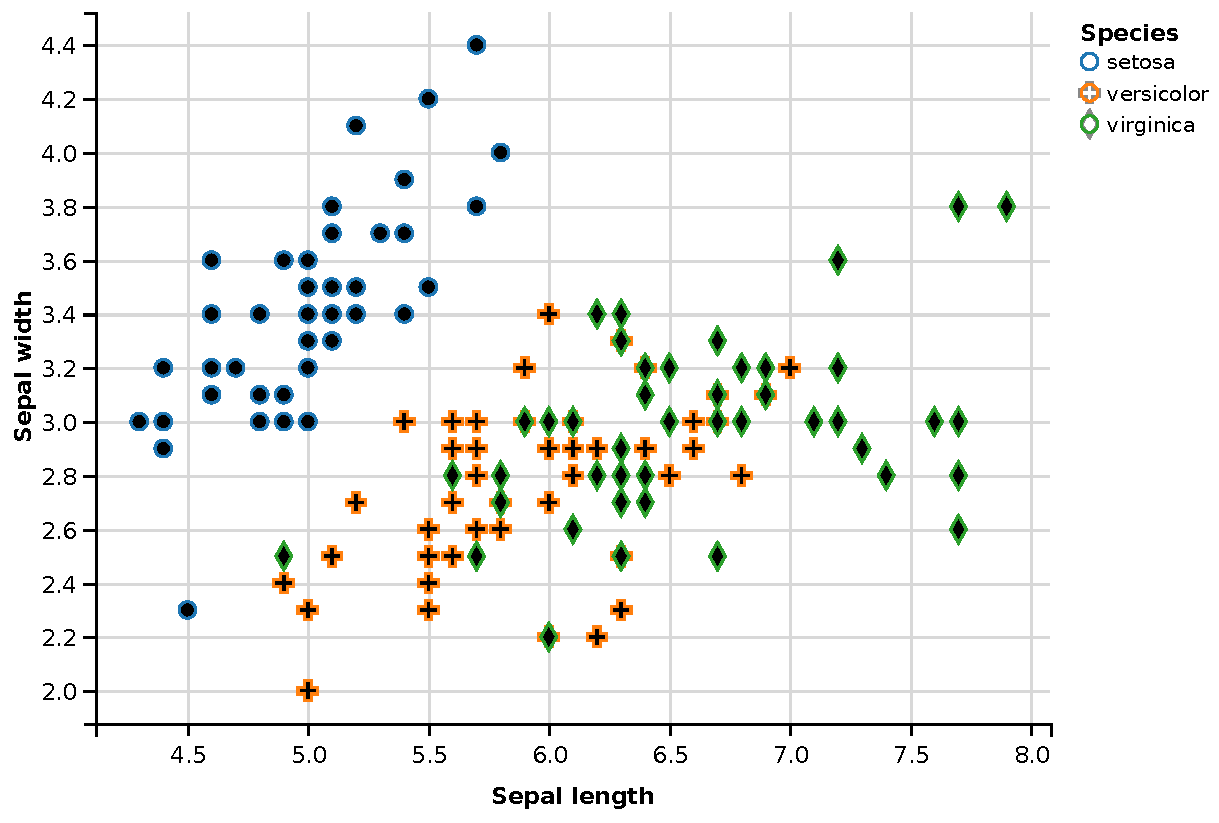
\includegraphics[scale=0.5]{plotsepalwidthsepallength}
    \caption{Populacja kwiatów irysów w zależności od szerokości i długości płatka kwiatu}
    \label{fig:plotsepalwidthsepallength}
\end{figure}

Stosując algorytmy uczenia nienadzorowanego, nie wiemy w jaki sposób klasyfikować dane trenujące. W tym celu możemy 
wykorzystać algorytm k-means\cite{coates2012learning}, który na podstawie określonych cech grupuje dane w podaną liczbę 
klastrów.
Poddając przedstawione dane działaniu algorytmu k-means, uzyskujemy wynik przedstawiony na rys. \ref{fig:cluster2} oraz 
rys. \ref{fig:cluster3}.


\begin{figure}[h!]
    \centering
    \textbf{Wynik działania algorytmu k-means}\par\medskip
    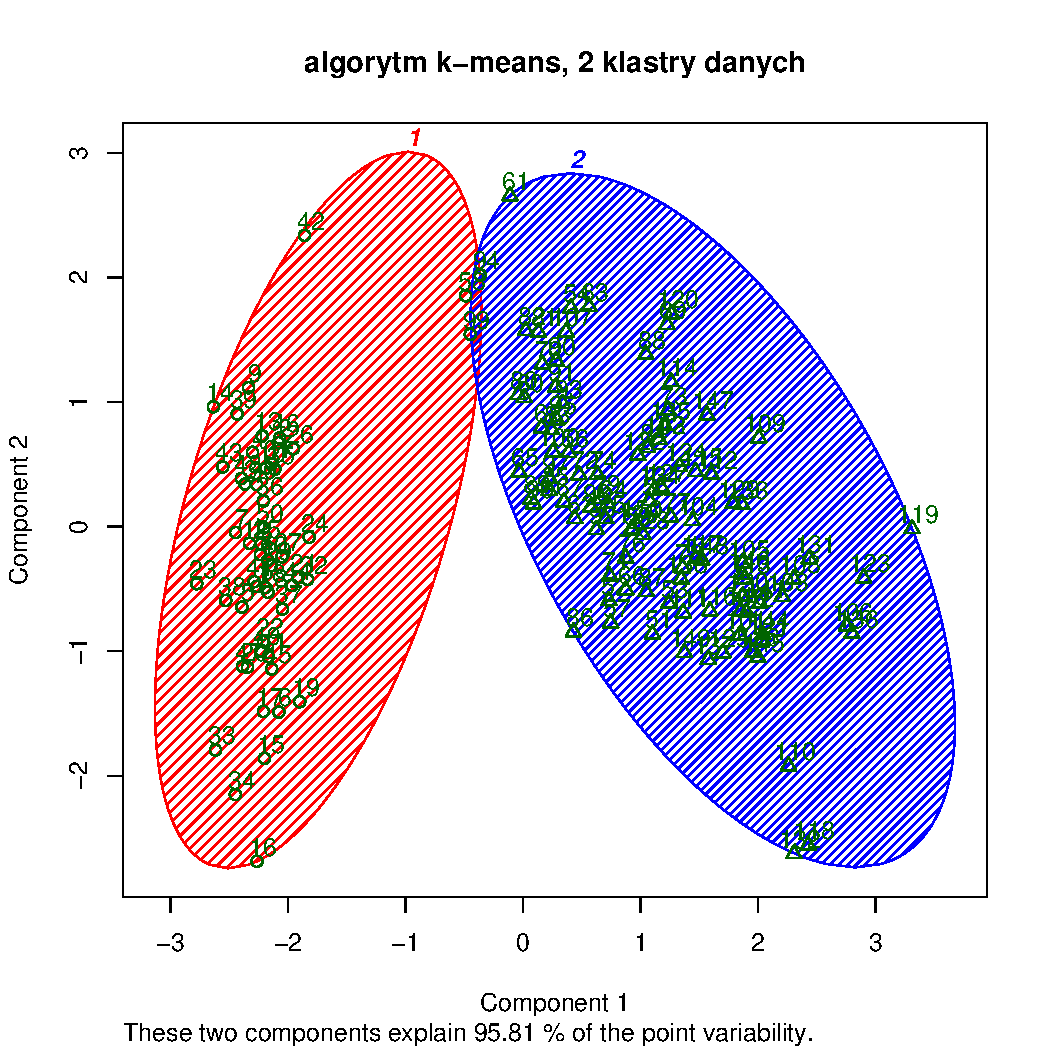
\includegraphics[scale=0.5]{cluster2}
    \caption{Wynik działania algorytmu klasteryzacji k-means dla 2 klastrów kwiatów irysów w zależności od szerokości i 
długości płatka kwiatu}
    \label{fig:cluster2}
\end{figure}

\begin{figure}[h!]
    \centering
    \textbf{Wynik działania algorytmu k-means}\par\medskip
    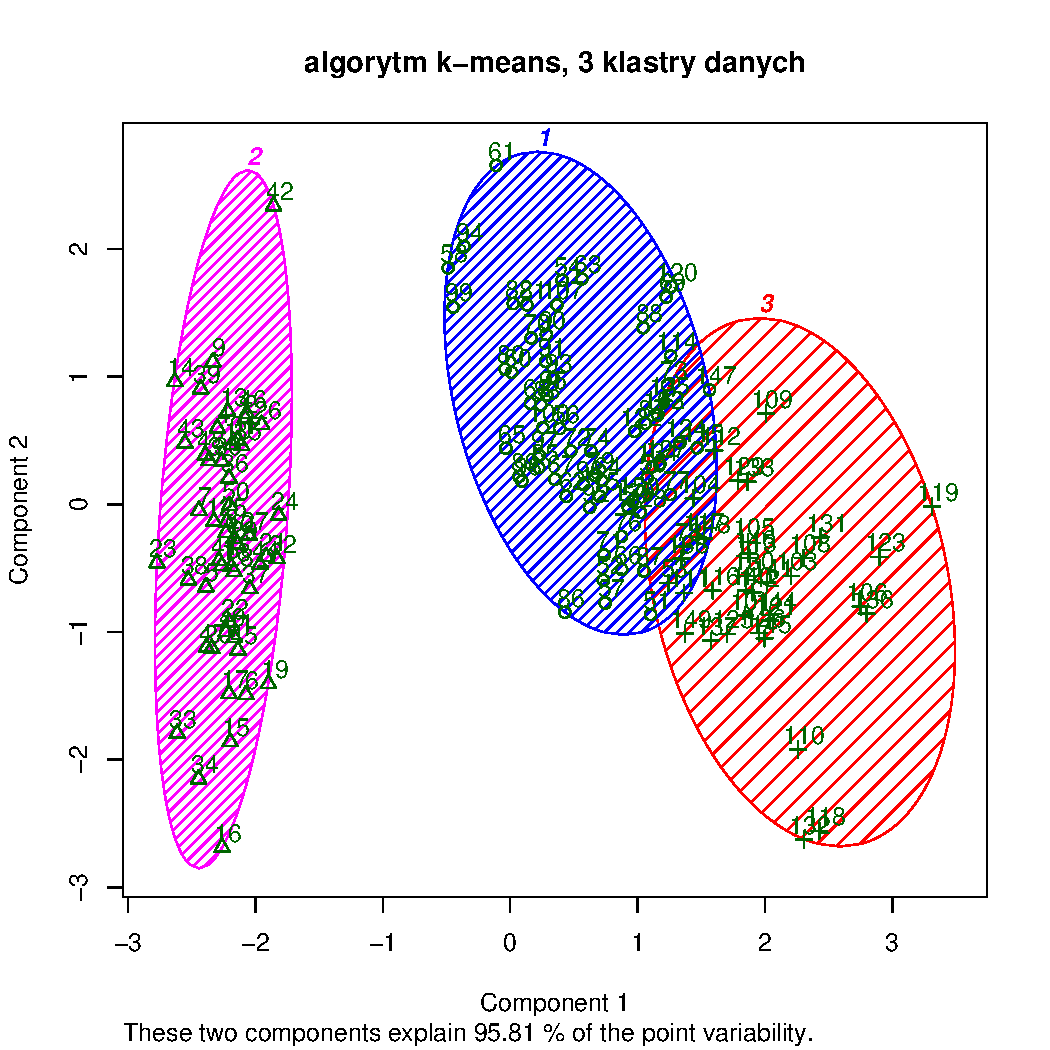
\includegraphics[scale=0.4]{cluster3}
    \caption{Wynik działania algorytmu klasteryzacji k-means dla 3 klastrów kwiatów irysów w zależności od szerokości i 
długości płatka kwiatu}
    \label{fig:cluster3}
\end{figure}


Na rys. \ref{fig:cluster2} można zaobserwować, że algorytm zadziała z dużą skutecznością rozróżniając pomiędzy dwoma 
gatunkami dla dwóch klastrów, tj. pomiędzy gatunkiem setosa, a gatunkami versicolor i virginica, jednak algorytm będzie 
miał problem rozróżnić pomiędzy gatunkami versicolor i virginica.
W tym celu można zbiór podzielić na trzy klastry jak na rys.\ref{fig:cluster3}, ale nie gwarantuje to 
wystarczającej skuteczności przydziału. \\
Tym samym można zaobserwować, że gatunek versicolor i virginica nie są 
rozróżnialne, używając przedstawionych danych wejściowych.\\
Rozważając sytuacje, w której dodana by została duża liczba dodatkowych wpisów, różnych od aktualnych danych, 
można by było zaobserwować pojawienie się kolejnego klastra danych, co oznacza pojawienie się nowego gatunku kwiatu.


\subsection{Uczenie ze wzmocnieniem}
\label{subsec:uczeniezewzmocnieniem}

Uczenie ze wzmocnieniem jest obszarem uczenia maszynowego, w którym inteligentny agent wykonując akcję w otoczeniu otrzymuje odpowiednią nagrodę.
Robot decyduje jaka akcja zostanie wykonana na podstawie istniejącej polityki. Algorytmy uczenia ze wzmocnieniem nie 
wymagają danych trenujących by wykonać swoje zadanie. Na podstawie wiedzy o stanie otoczenia, możliwych do wykonania 
akcji w danym stanie oraz funkcji nagrody, która agent otrzymuje za wykonanie danych akcji, robot, ucząc się metodą 
prób i błędów odkrywa sposoby wybierania kolejnych akcji (polityki) tak, aby osiągnąć swój cel.

\begin{figure}[h]
    \centering
    \textbf{Uczenie ze wzmocnieniem}\par\medskip
    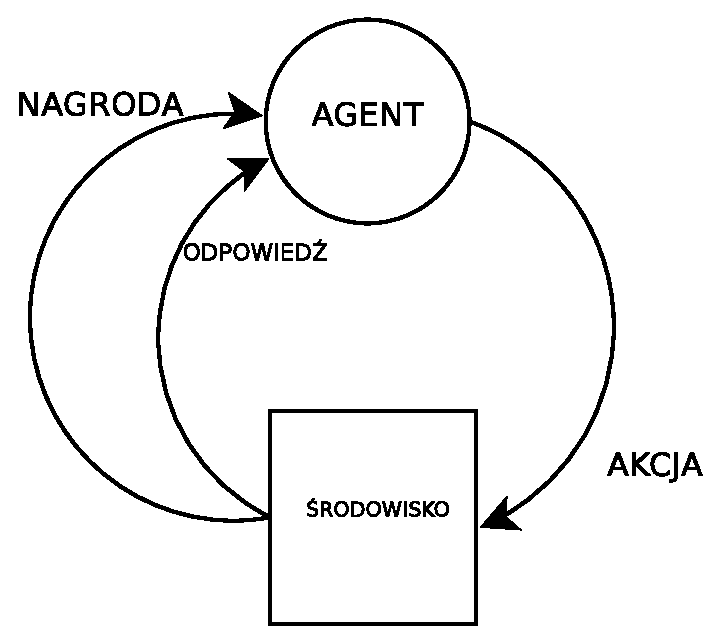
\includegraphics[scale=0.8]{DIAGRAMreinforcementlearning}
    \caption{Schemat uczenia ze wzmocnieniem}
    \label{fig:DIAGRAMreinforcementlearning}
\end{figure}

Na rys. \ref{fig:DIAGRAMreinforcementlearning} przedstawiono schemat współpracy agenta ze środowiskiem. Agent 
podejmując akcję w otoczeniu dostaje nagrodę za podjętą decyzję w danym stanie, oraz informacje o nowym, aktualnym 
stanie środowiska (otoczenie może ulec zmianie po wykonaniu przez robota akcji).

Algorytmy uczenia ze wzmocnieniem dotyczą specyficznych zadań występujących w uczeniu maszynowym. Problem polega na 
odnalezieniu przez agenta optymalnej akcji do wykonania na podstawie wiedzy o aktualnym jego stanie. W przypadku, 
gdy to działanie jest powtórzone, możemy mówić o MDP (Procesy decyzyjne Markowa).

Procesem decyzyjnym Markowa nazywamy model środowiska w algorytmach uczenia ze wzmocnieniem, oznaczamy go jako:\\
$$MDP = (S, A, P(s, s'), R(r, r'), \gamma)$$
gdzie
\begin{enumerate}
 \item $S$ to zbiór stanów
 \item $A$ zbiór możliwych akcji
 \item $P(s, s')$ prawdopodobieństwo przejścia do stanu $s'$ ze stanu $s$ po wykonaniu akcji $a$, w czasie $t$
 \item $R(r, r')$ nagroda po przejściu do stanu $s'$ ze stanu $s$
 \item $\gamma$ współczynnik regulujący stosunek między nagrodami przewidywanymi w późniejszym czasie i 
otrzymywanymi aktualnie, $0 < \gamma < 1$
\end{enumerate}

Zadaniem MDP jest uzyskanie takiej polityki robota, która zmaksymalizuje sumę otrzymywanych nagród.

$$\sum\limits_{t=0}^\infty \gamma^{t} R_{a_{t}}(s_{t}, s_{t+1})$$

Algorytmy uczenia ze wzmocnieniem znalazły zastosowanie między innymi w implementacji autonomicznego 
helikoptera\cite{abbeel2007application}, udoskonaleniu działania windy\cite{barto1996improving}, usprawnienia 
sygnalizacji świetlnej\cite{wiering2000multi} czy budowie inteligentnego robota\cite{kimura2001reinforcement}.

\subsubsection{Q-learning}
\label{subsubsec:qlearning}

Algorytm Q-learning \cite{watkins1992q} jest off-policy
\subsection{SARSA}


\section{Podsumowanie}

Uczenie nienadzorowane posiada tę przewagę nad uczniem nadzorowanym, że nie wymaga oznaczenia danych trenujących 
oraz potrafi wykryć ukryte zależności pomiędzy cechami przykładów. Jednak w odróżnieniu od obydwu metod, uczenie ze 
wzmacnianiem jest odmienne w tym, że nie wymaga podawania jakichkolwiek danych przykładowych, a jedynie na podstawie 
zdefiniowanych nagród i akcji, agent uczy się odpowiedniego działania.
By zaimplementować robota uczącego się wykonywania akcji w otoczeniu wybrano implementacje metod uczenia ze 
wzmacnianiem, ze względu na charakterystykę środowiska odpowiadającą wymaganiom procesów decyzyjnych Markowa.












